\documentclass[letterpaper, 10 pt, conference]{ieeeconf}  % Comment this line out
                                                          % if you need a4paper
%\documentclass[a4paper, 10pt, conference]{ieeeconf}      % Use this line for a4
                                                          % paper

\IEEEoverridecommandlockouts                              % This command is only
                                                          % needed if you want to
                                                          % use the \thanks command
\overrideIEEEmargins
% See the \addtolength command later in the file to balance the column lengths
% on the last page of the document



% The following packages can be found on http:\\www.ctan.org
%\usepackage{graphics} % for pdf, bitmapped graphics files
%\usepackage{epsfig} % for postscript graphics files
%\usepackage{mathptmx} % assumes new font selection scheme installed
%\usepackage{times} % assumes new font selection scheme installed

\usepackage{amsmath} % assumes amsmath package installed
\usepackage{amssymb}  % assumes amsmath package installed
\usepackage{pgfplots}

\newcommand{\picalign}{\vspace{1ex}\hspace{-3ex}}

\newcommand{\EE}{\mathbb{E}}
\newcommand{\yh}{\hat y}
\newcommand{\Iff}{\Leftrightarrow}
\newcommand{\eu}{\mathrm{EU}}


\title{\LARGE \bf
Coalitions either build non-agents or agents \\
that care about things the coalition doesn't}

%\author{ \parbox{3 in}{\centering Huibert Kwakernaak*
%         \thanks{*Use the $\backslash$thanks command to put information here}\\
%         Faculty of Electrical Engineering, Mathematics and Computer Science\\
%         University of Twente\\
%         7500 AE Enschede, The Netherlands\\
%         {\tt\small h.kwakernaak@autsubmit.com}}
%         \hspace*{ 0.5 in}
%         \parbox{3 in}{ \centering Pradeep Misra**
%         \thanks{**The footnote marks may be inserted manually}\\
%        Department of Electrical Engineering \\
%         Wright State University\\
%         Dayton, OH 45435, USA\\
%         {\tt\small pmisra@cs.wright.edu}}
%}

\author{Andrew Critch$^{1,2}$% <-this % stops a space
\thanks{$^{1}$Machine Intelligence Research Institute, and UC Berkeley}%
\thanks{$^{1}$UC Berkeley, Center for Human Compatible AI}%
}


\begin{document}

\maketitle
\thispagestyle{empty}
\pagestyle{empty}


%%%%%%%%%%%%%%%%%%%%%%%%%%%%%%%%%%%%%%%%%%%%%%%%%%%%%%%%%%%%%%%%%%%%%%%%%%%%%%%%
\begin{abstract}
These are just plotting examples
\end{abstract}


%%%%%%%%%%%%%%%%%%%%%%%%%%%%%%%%%%%%%%%%%%%%%%%%%%%%%%%%%%%%%%%%%%%%%%%%%%%%%%%%
\section{INTRODUCTION}


\picalign
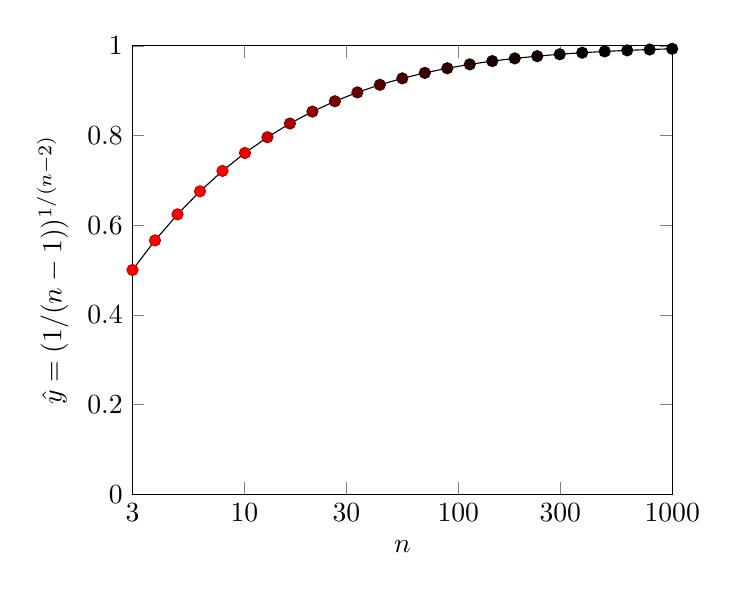
\begin{tikzpicture}
  \begin{axis}[
  	colormap={bw}{rgb(0cm)=(1,0,0); rgb(1cm)=(1,0,0); gray(2cm)=(0)},
  	xmode=log,
    xlabel=$n$, 
    xtick={3,10,30,100,300,1000},
    xticklabels={$3$,$10$,$30$,$100$,$300$,$1000$},
    ylabel={$\yh = (1/(n-1))^{1/(n-2)}$},
    xmin=3, xmax=1000, xstep=1, 
    ymin=0, ymax=1
  ] 
    \addplot[scatter,domain=3:1000]{(1/(x-1))^(1/(x-2))}; 
  \end{axis}
\end{tikzpicture}



\picalign
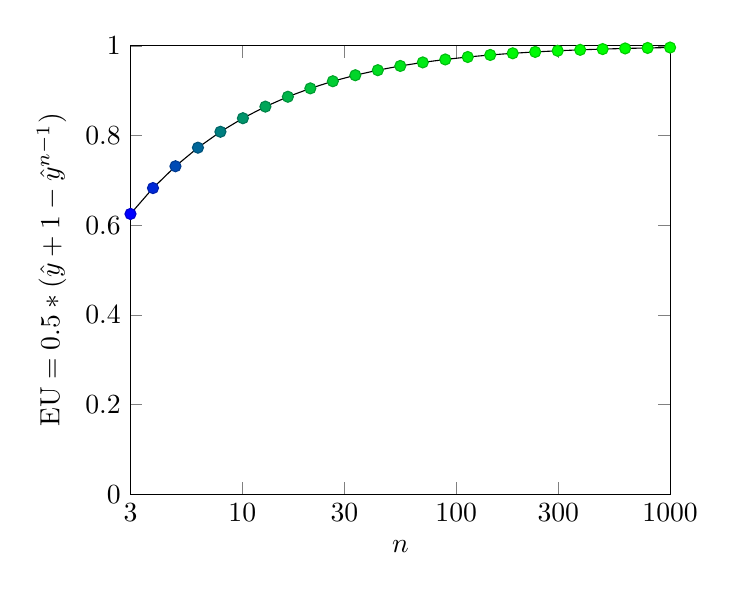
\begin{tikzpicture}
  \begin{axis}[
  	colormap={bw}{rgb(0cm)=(0,0,1); rgb(1cm)=(0,1,0)},
  	xmode=log,
    xlabel=$n$, 
    xtick={3,10,30,100,300,1000},
    xticklabels={$3$,$10$,$30$,$100$,$300$,$1000$},
    ylabel={$\eu = 0.5*(\yh + 1 - \yh^{n-1})$},
    xmin=3, xmax=1000, xstep=1, 
    ymin=0, ymax=1
  ] 
    \addplot[scatter,domain=3:1000]{0.5*((1/(x-1))^(1/(x-2))+1-(1/(x-1))^((x-1)/(x-2))}; 
  \end{axis}
\end{tikzpicture}

\picalign
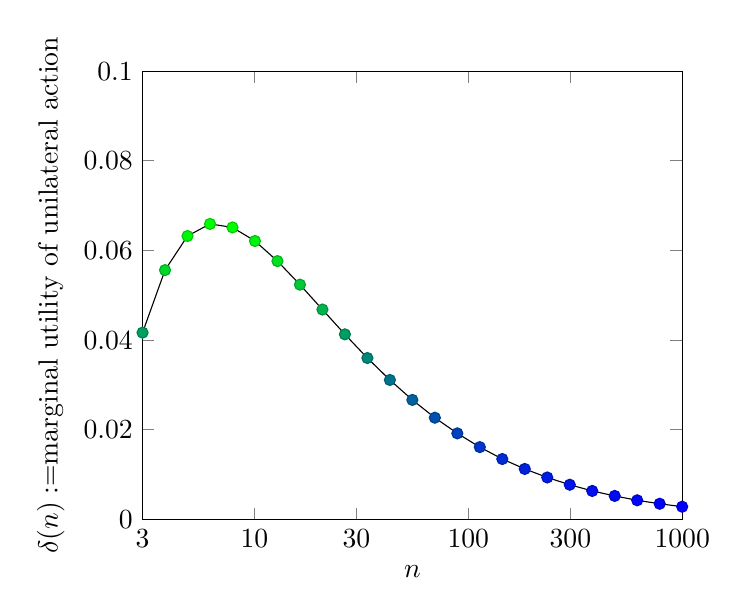
\begin{tikzpicture}
  \begin{axis}[
  	colormap={bw}{rgb(0cm)=(0,0,1); rgb(1cm)=(0,1,0)},
  	xmode=log,
	y tick label style={/pgf/number format/fixed},
    xlabel=$n$, 
    xtick={3,10,30,100,300,1000},
    xticklabels={$3$,$10$,$30$,$100$,$300$,$1000$},
    ylabel={$\delta(n):=$marginal utility of unilateral action},
    xmin=3, xmax=1000, xstep=1, 
    ymin=0, ymax=0.1
  ] 
    \addplot[scatter,domain=3:1000]{1-1/x -(0.5*((1/(x-1))^(1/(x-2))+1-(1/(x-1))^((x-1)/(x-2)))}; 
  \end{axis}

\end{tikzpicture}


\addtolength{\textheight}{-12cm}   % This command serves to balance the column lengths
                                  % on the last page of the document manually. It shortens
                                  % the textheight of the last page by a suitable amount.
                                  % This command does not take effect until the next page
                                  % so it should come on the page before the last. Make
                                  % sure that you do not shorten the textheight too much.

%%%%%%%%%%%%%%%%%%%%%%%%%%%%%%%%%%%%%%%%%%%%%%%%%%%%%%%%%%%%%%%%%%%%%%%%%%%%%%%%



%%%%%%%%%%%%%%%%%%%%%%%%%%%%%%%%%%%%%%%%%%%%%%%%%%%%%%%%%%%%%%%%%%%%%%%%%%%%%%%%



%%%%%%%%%%%%%%%%%%%%%%%%%%%%%%%%%%%%%%%%%%%%%%%%%%%%%%%%%%%%%%%%%%%%%%%%%%%%%%%%
\section*{APPENDIX}

Appendixes should appear before the acknowledgment.

\section*{ACKNOWLEDGMENT}

%%%%%%%%%%%%%%%%%%%%%%%%%%%%%%%%%%%%%%%%%%%%%%%%%%%%%%%%%%%%%%%%%%%%%%%%%%%%%%%%

References are important to the reader; therefore, each citation must be complete and correct. If at all possible, references should be commonly available publications.



\begin{thebibliography}{99}

\bibitem{Bo16} Bostrom, N., Douglas, T., and Sandberg, A. (2016). The Unilateralist’s Curse and the Case for a Principle of Conformity. Social Epistemology, 30(4), 350-371.

\end{thebibliography}




\end{document}
